\subsection{Modelo M/M/1 en AnyLogic}

\begin{figure}[H]
  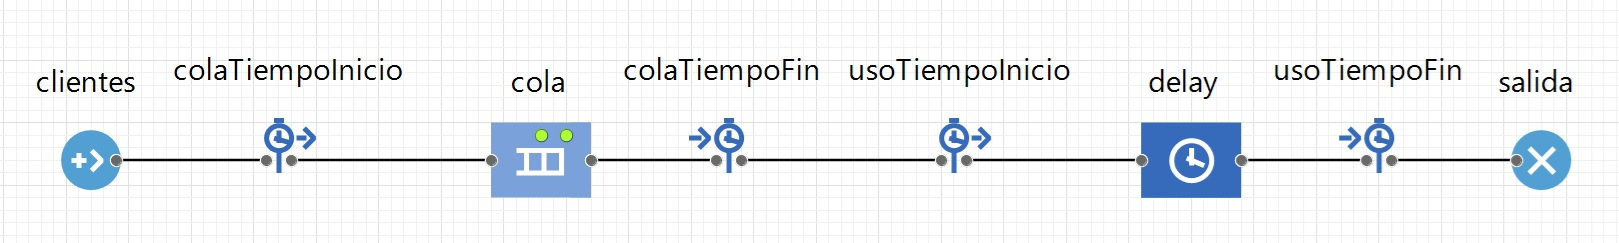
\includegraphics[width=\linewidth]{images/anylogic-colas-modelo}
  \caption{Bloques del modelo M/M/1 en Anylogic.}
\end{figure}

Para analizar el rendimiento del modelo, variamos la tasa de arribos ($T_a$) en base a la tasa de servicio ($T_s$), y
la capacidad de la cola ($cap$).

Realizaremos 10 simulaciones de 1000 clientes cada una y promediamos los siguientes estadísticos:
\begin{itemize}
    \item Promedio de clientes en el sistema ($q(n)+u(n)$)
    \item Cantidad de clientes en cola en promedio ($q(n)$)
    \item Demora promedio esperada en cola ($d(n)$)
    \item Tiempo promedio en el sistema ($d(n)+s(n)$)
    \item Ocupación del servidor ($u(n)*100\%$)
    \item Probabilidad de denegación del servicio. ($p(den)$)
    \item Probabilidad de encontrar n clientes en cola. ($p(Q(t)=n)\times100\%$)
\end{itemize}

Los primeros 5 fueron tabulados y el último fue graficado.

\subsubsection[cap = 0]{$cap = 0$}

Los parámetros $d(n)$, $q(n)$ y $p(Q(t)=n)\times100\%$ no aplican cuando la capacidad de la cola es 0.
El promedio de clientes en sistema es en este caso, equivalente al factor de uso del servicio.

\begin{tabular}{||c||c|c|c||}
    \hline \hline
    $\frac{T_a}{T_s}\times100\%$ [\%] & $d(n)+s(n)$ [min] & $u(n)\times100\%$ [\%] & $p(den)$ [\%] \\
    \hline \hline
    25 & $2,005$ & $19,823$ & $19,46$ \\
    \hline
    50 & $2,059$ & $33,656$ & $34,09$ \\
    \hline
    75 & $1,93$ & $42,212$ & $41,65$ \\
    \hline
    100 & $1,985$ & $49,165$ & $50,12$ \\
    \hline
    125 & $2,004$ & $55,434$ & $55,15$ \\
    \hline \hline
\end{tabular}

\subsubsection[cap = 2]{$cap = 2$}

\begin{tabular}{||c||c|c|c|c|c|c||}
    \hline \hline
    $\frac{T_a}{T_s}\times100\%$ [\%] & $q(n)+u(n)$ [min] & $q(n)$ [clientes] & $d(n)$ [min] & $d(n)+s(n)$ [min] & $u(n)\times100\%$ [\%] & $p(den)$ [\%] \\
    \hline \hline
    25 & $0,313$ & $0,068$ & $0,548$ & $2,54$ & $24,546$ & $1,26$ \\
    \hline
    50 & $0,739$ & $0,266$ & $1,148$ & $3,186$ & $47,27$ & $6,39$ \\
    \hline
    75 & $1,168$ & $0,524$ & $1,65$ & $3,681$ & $64,373$ & $15,71$ \\
    \hline
    100 & $1,499$ & $0,748$ & $2,014$ & $4,039$ & $75,164$ & $25,3$ \\
    \hline
    125 & $1,756$ & $0,934$ & $2,26$ & $4,246$ & $82,168$ & $32,93$ \\
    \hline \hline
\end{tabular}

\begin{figure}[H]
  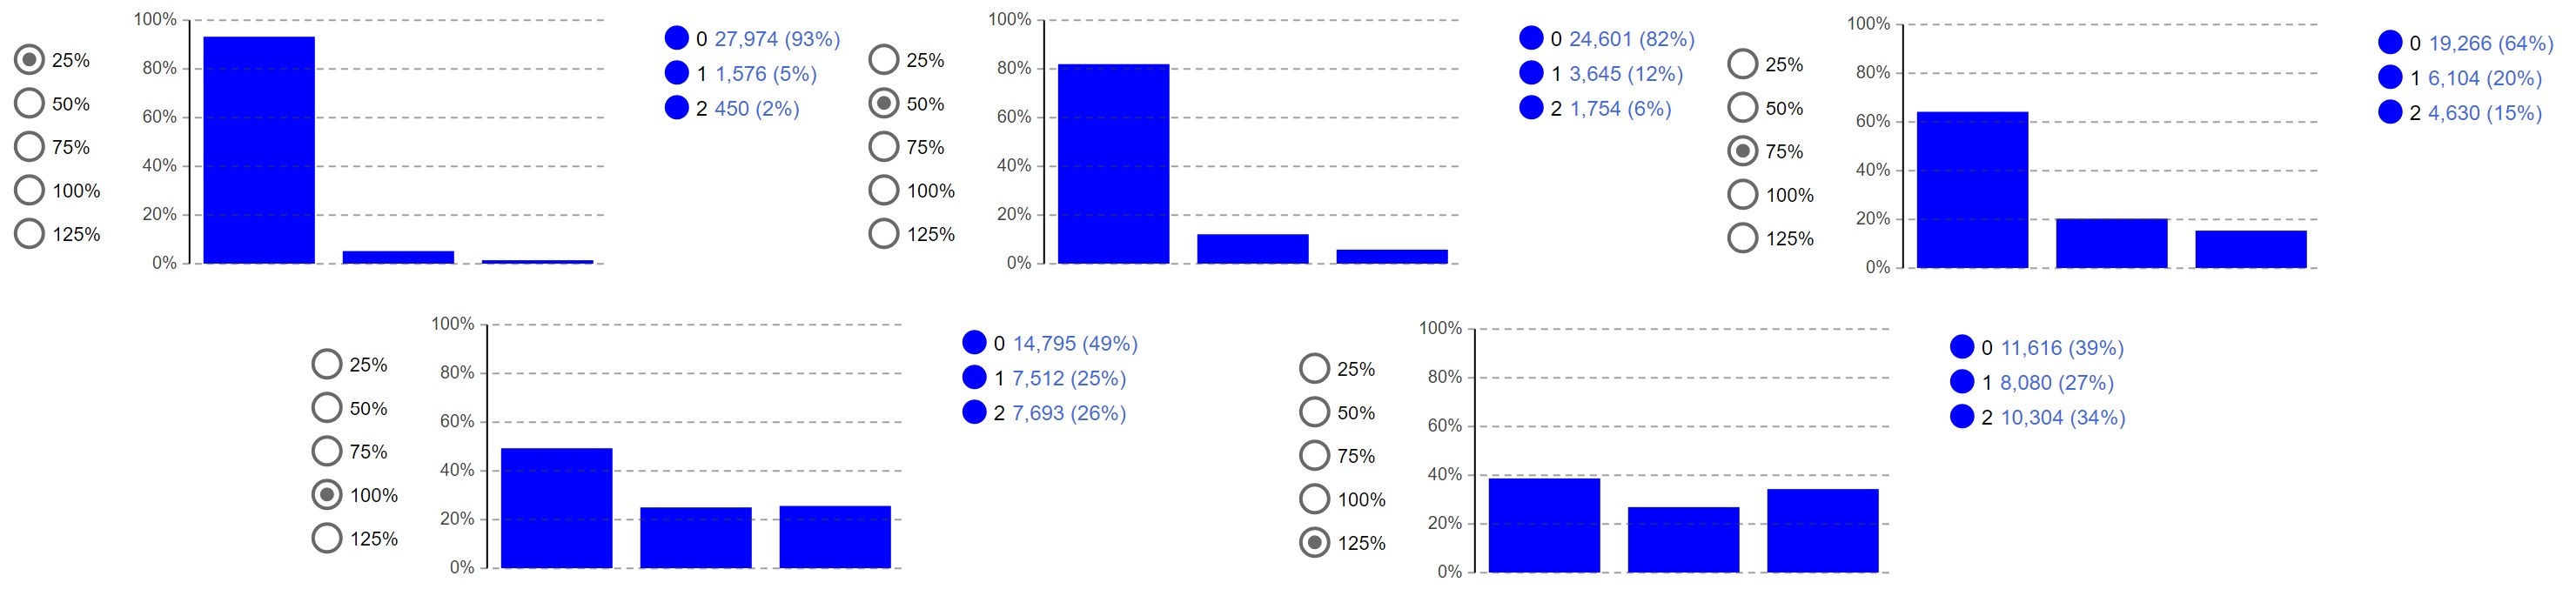
\includegraphics[width=\linewidth]{images/anylogic-colas-2}
  \caption{Probabilidad de encontrar n clientes en cola.}
\end{figure}

\subsubsection[cap = 5]{$cap = 5$}

\begin{tabular}{||c||c|c|c|c|c|c||}
    \hline \hline
    $\frac{T_a}{T_s}\times100\%$ [\%] & $q(n)+u(n)$ [min] & $q(n)$ [clientes] & $d(n)$ [min] & $d(n)+s(n) [min]$ & $u(n)\times100\%$ [\%] & $p(den)$ [\%] \\
    \hline \hline
    25 & $0,326$ & $0,079$ & $0,634$ & $2,069$ & $24,672$ & $0,01$ \\
    \hline
    50 & $0,917$ & $0,424$ & $1,7$ & $3,681$ & $49,263$ & $0,85$ \\
    \hline
    75 & $1,882$ & $1,18$ & $3,318$ & $5,289$ & $70,119$ & $4,9$ \\
    \hline
    100 & $3,122$ & $2,253$ & $5,234$ & $7,254$ & $86,914$ & $14,19$ \\
    \hline
    125 & $3,847$ & $2,917$ & $6,267$ & $8,266$ & $93,034$ & $25,23$ \\
    \hline \hline
\end{tabular}

\begin{figure}[H]
  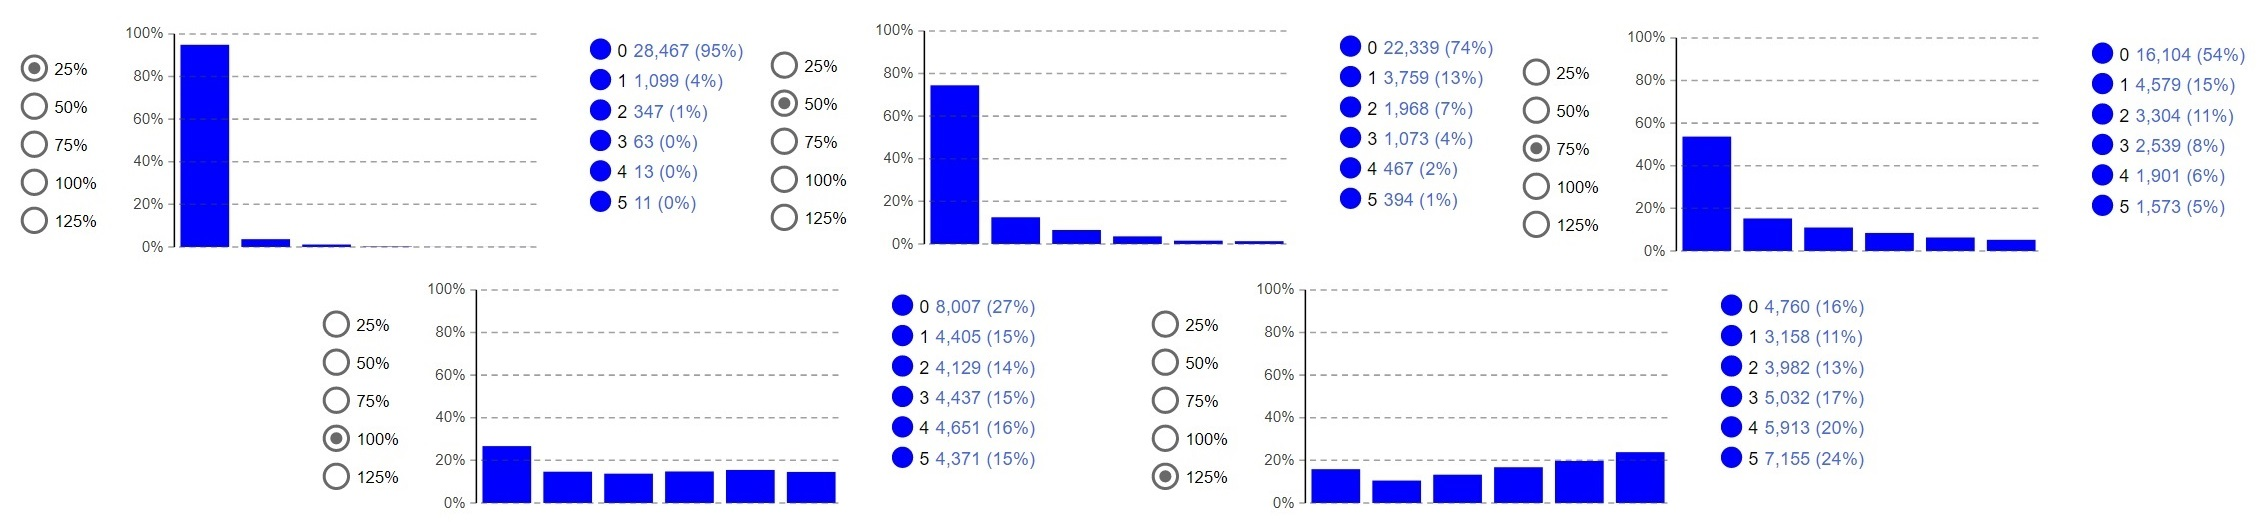
\includegraphics[width=\linewidth]{images/anylogic-colas-5}
  \caption{Probabilidad de encontrar n clientes en cola.}
\end{figure}

\subsubsection[cap = 10]{$cap = 10$}

\begin{tabular}{||c||c|c|c|c|c|c||}
    \hline \hline
    $\frac{T_a}{T_s}\times100\%$ [\%] & $q(n)+u(n)$ [min] & $q(n)$ [clientes] & $d(n)$ [min] & $d(n)+s(n) [min]$ & $u(n)\times100\%$ [\%] & $p(den)$ [\%] \\
    \hline \hline
    25 & $0,325$ & $0,08$ & $0,648$ & $2,631$ & $24,52$ & $0$ \\
    \hline
    50 & $1,032$ & $0,534$ & $2,15$ & $4,159$ & $49,816$ & $0,08$ \\
    \hline
    75 & $2,314$ & $1,593$ & $4,351$ & $6,332$ & $72,183$ & $0,64$ \\
    \hline
    100 & $5,294$ & $4,382$ & $9,62$ & $11,623$ & $91,217$ & $8.13$ \\
    \hline
    125 & $7,582$ & $6,606$ & $13.329$ & $15,296$ & $97.504$ & $19,65$ \\
    \hline \hline
\end{tabular}

\begin{figure}[H]
  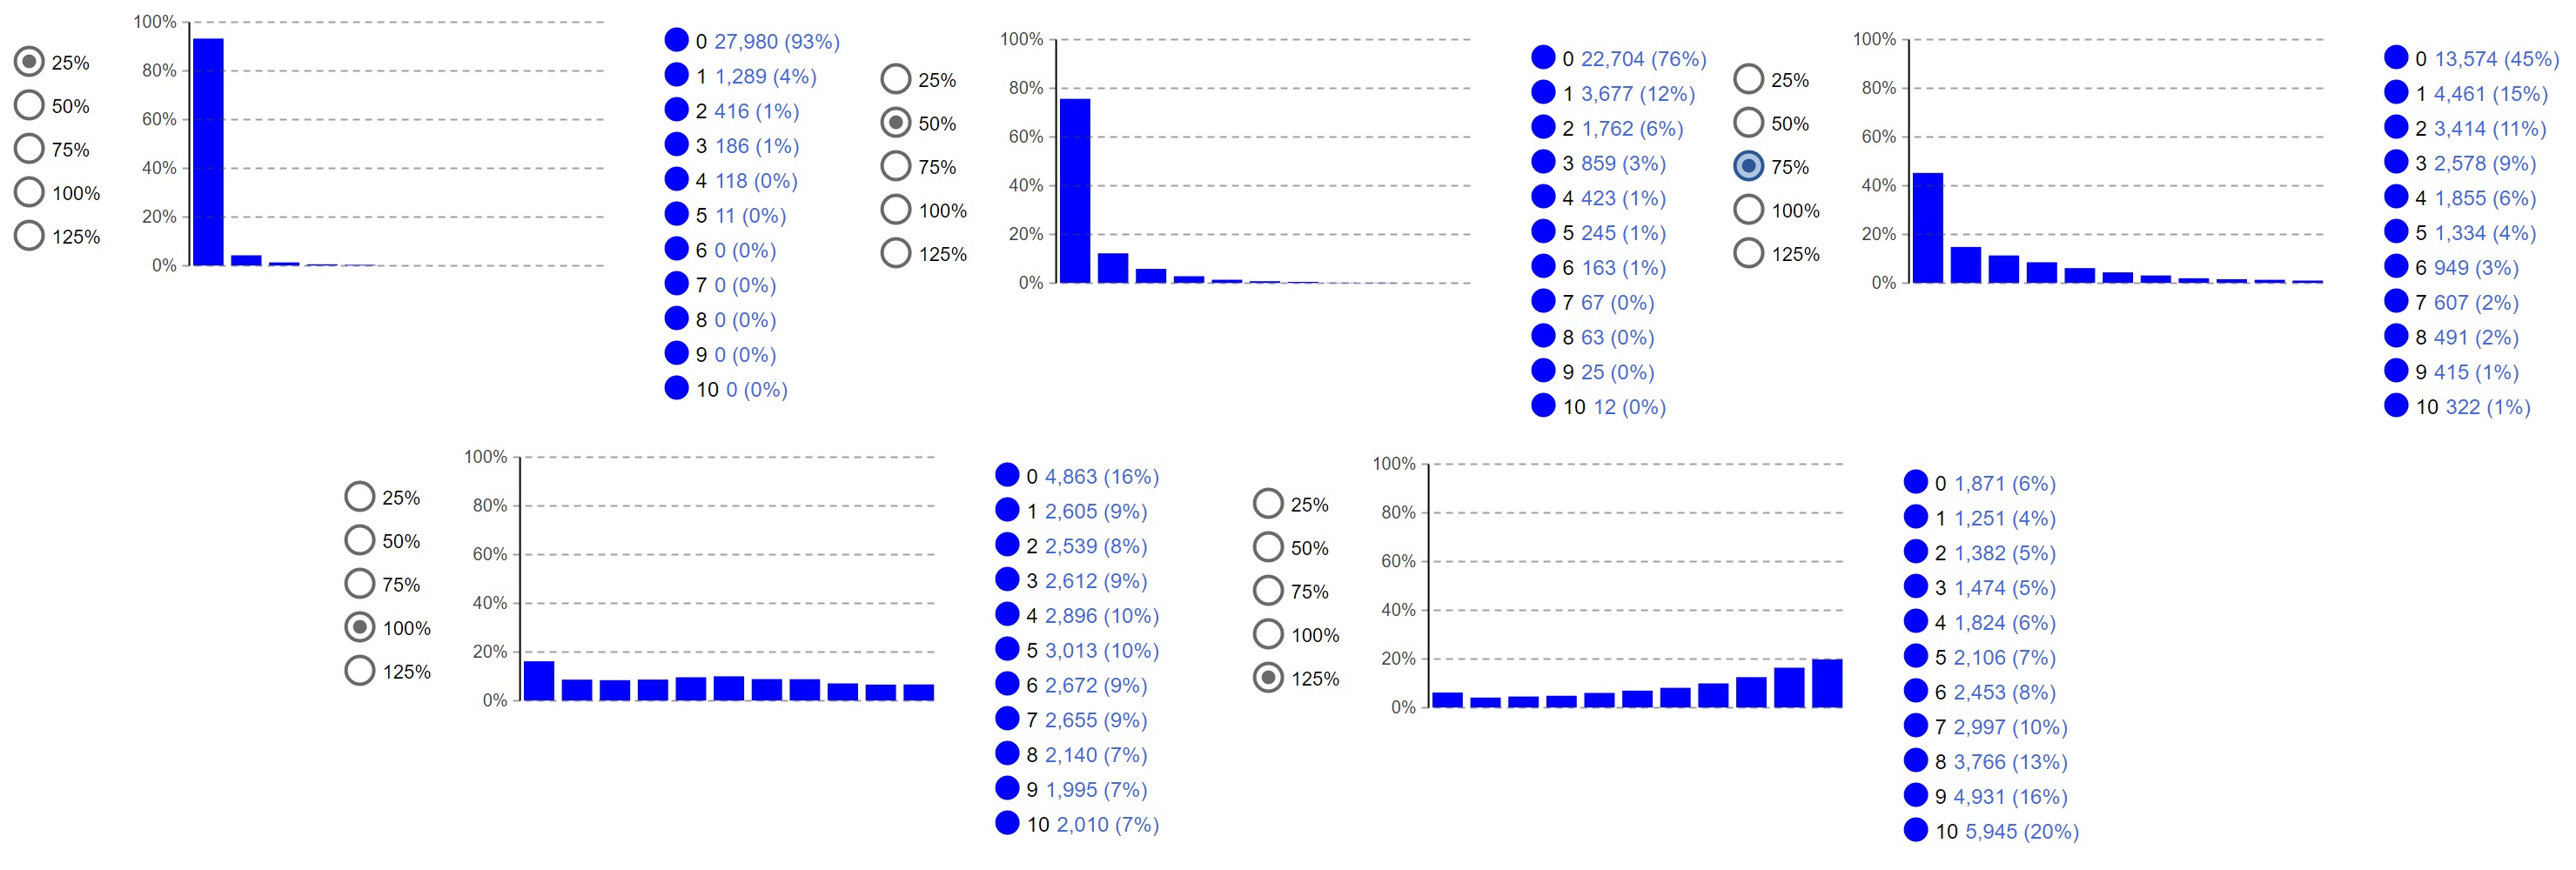
\includegraphics[width=\linewidth]{images/anylogic-colas-10}
  \caption{Probabilidad de encontrar n clientes en cola.}
\end{figure}

\subsubsection[cap = 50]{$cap = 50$}

\begin{tabular}{||c||c|c|c|c|c|c||}
    \hline \hline
    $\frac{T_a}{T_s}\times100\%$ [\%] & $q(n)+u(n)$ [min] & $q(n)$ [clientes] & $d(n)$ [min] & $d(n)+s(n) [min]$ & $u(n)\times100\%$ [\%] & $p(den)$ [\%] \\
    \hline \hline
    25 & $0,335$ & $0,085$ & $0,679$ & $2,686$ & $25,007$ & $0$ \\
    \hline
    50 & $1,039$ & $0,532$ & $2,099$ & $4,11$ & $50,7$ & $0$ \\
    \hline
    75 & $3,116$ & $2,368$ & $6,341$ & $8,358$ & $74,8$ & $0$ \\
    \hline
    100 & $22,932$ & $21,957$ & $45,615$ & $47,631$ & $97,42$ & $0,8$ \\
    \hline
    125 & $39,365$ & $38,37$ & $75,431$ & $77,386$ & $99,539$ & $13,41$ \\
    \hline \hline
\end{tabular}

\begin{figure}[H]
  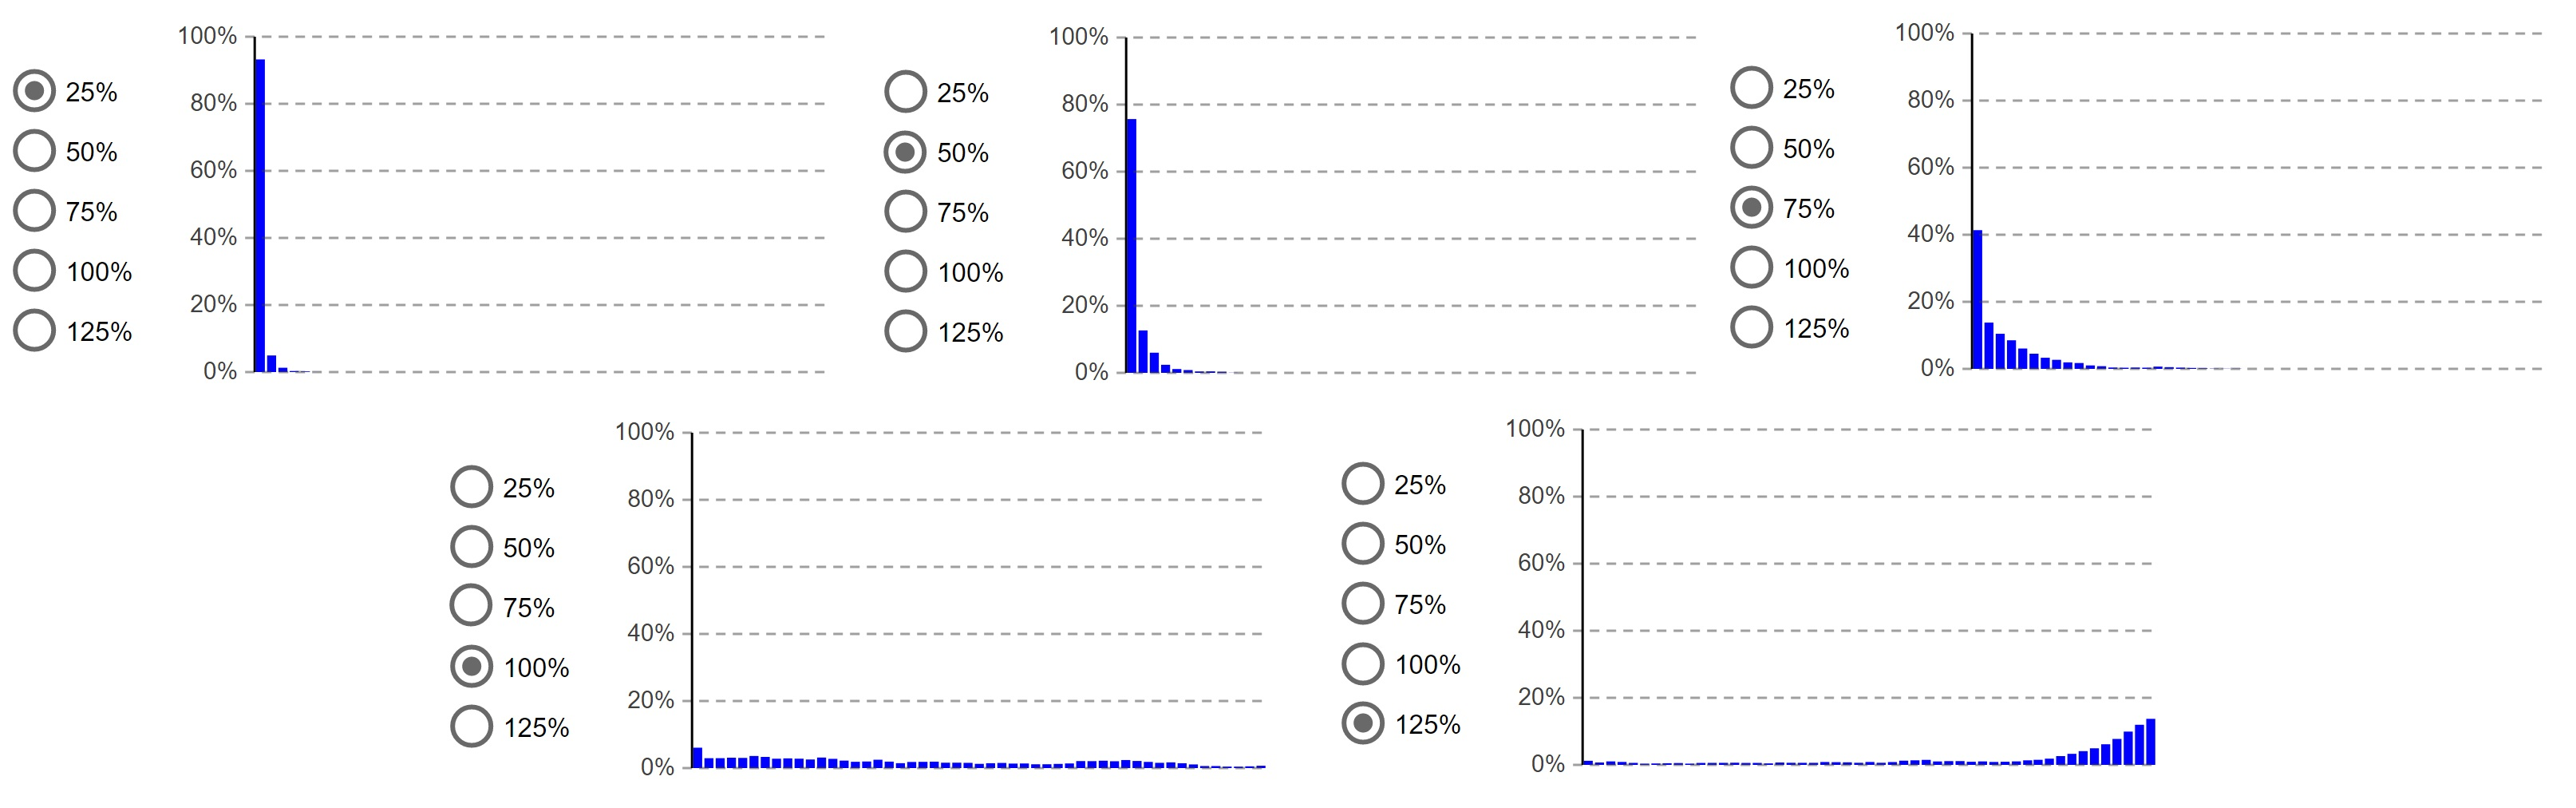
\includegraphics[width=\linewidth]{images/anylogic-colas-50}
  \caption{Probabilidad de encontrar n clientes en cola.}
\end{figure}
